% title: response.tex
% description: Response to eLife Reviewers
% author: twab

% USAGE: 
% to compile this document:
%    R  >>> knitr::knit("response.Rnw")
%    sh >>> pdflatex response.tex





% latex document setup

\documentclass[11pt]{elife}\usepackage[]{graphicx}\usepackage[]{color}
% maxwidth is the original width if it is less than linewidth
% otherwise use linewidth (to make sure the graphics do not exceed the margin)
\makeatletter
\def\maxwidth{ %
  \ifdim\Gin@nat@width>\linewidth
    \linewidth
  \else
    \Gin@nat@width
  \fi
}
\makeatother

\definecolor{fgcolor}{rgb}{0.345, 0.345, 0.345}
\newcommand{\hlnum}[1]{\textcolor[rgb]{0.686,0.059,0.569}{#1}}%
\newcommand{\hlstr}[1]{\textcolor[rgb]{0.192,0.494,0.8}{#1}}%
\newcommand{\hlcom}[1]{\textcolor[rgb]{0.678,0.584,0.686}{\textit{#1}}}%
\newcommand{\hlopt}[1]{\textcolor[rgb]{0,0,0}{#1}}%
\newcommand{\hlstd}[1]{\textcolor[rgb]{0.345,0.345,0.345}{#1}}%
\newcommand{\hlkwa}[1]{\textcolor[rgb]{0.161,0.373,0.58}{\textbf{#1}}}%
\newcommand{\hlkwb}[1]{\textcolor[rgb]{0.69,0.353,0.396}{#1}}%
\newcommand{\hlkwc}[1]{\textcolor[rgb]{0.333,0.667,0.333}{#1}}%
\newcommand{\hlkwd}[1]{\textcolor[rgb]{0.737,0.353,0.396}{\textbf{#1}}}%
\let\hlipl\hlkwb

\usepackage{framed}
\makeatletter
\newenvironment{kframe}{%
 \def\at@end@of@kframe{}%
 \ifinner\ifhmode%
  \def\at@end@of@kframe{\end{minipage}}%
  \begin{minipage}{\columnwidth}%
 \fi\fi%
 \def\FrameCommand##1{\hskip\@totalleftmargin \hskip-\fboxsep
 \colorbox{shadecolor}{##1}\hskip-\fboxsep
     % There is no \\@totalrightmargin, so:
     \hskip-\linewidth \hskip-\@totalleftmargin \hskip\columnwidth}%
 \MakeFramed {\advance\hsize-\width
   \@totalleftmargin\z@ \linewidth\hsize
   \@setminipage}}%
 {\par\unskip\endMakeFramed%
 \at@end@of@kframe}
\makeatother

\definecolor{shadecolor}{rgb}{.97, .97, .97}
\definecolor{messagecolor}{rgb}{0, 0, 0}
\definecolor{warningcolor}{rgb}{1, 0, 1}
\definecolor{errorcolor}{rgb}{1, 0, 0}
\newenvironment{knitrout}{}{} % an empty environment to be redefined in TeX

\usepackage{alltt}
\usepackage{amsmath}
\usepackage{amssymb}
\usepackage{amsthm}
\usepackage{ragged2e}
\usepackage{caption}
\usepackage{fancyhdr}
\usepackage{graphicx}
\usepackage{titlesec}
\usepackage{blkarray}
\usepackage{csquotes}

% location of figures
\graphicspath{ {./figs/} }


\title{Supplementary Methods\\
\small{Genetic Disruption of WASHC4 Drives Endo-lysosomal Dysfunction and \\
Cognitive-Movement Impairments in Mice and Humans}}


% Authors
\author[1\authfn{0}]{Jamie Courtland}
\author[1\authfn{0}]{Tyler W. A. Bradshaw}
\author[2]{Greg Waitt}
\author[2,3]{Erik J. Soderblom}
\author[2]{Tricia Ho}
\author[4]{Anna Rajab}
\author[5]{Ricardo Vancini}
\author[2\authfn{1}]{Il Hwan Kim}
\author[6]{Ting Huang}
\author[6]{Olga Vitek}
\author[3]{Scott H. Soderling}

\affil[1]{Department of Neurobiology, Duke University School of Medicine, 
Durham, NC 27710, USA}
\affil[2]{Proteomics and Metabolomics Shared Resource, 
Duke University School of Medicine, Durham, NC 27710, USA}
\affil[3]{Department of Cell Biology, Duke University School of Medicine, 
Durham, NC 27710, USA}
\affil[4]{Burjeel Hospital, VPS Healthcare, Muscat, Oman}
\affil[5]{Department of Pathology, Duke University School of Medicine, 
Durham, NC 27710, USA}
\affil[6]{Khoury College of Computer Sciences, Northeaster University,
Boston, MA 02115, USA}

\contrib[\authfn{0}]{These authors contributed equally to this work.}
\presentadd[\authfn{1}]{Department of Anatomy and Neurobiology, 
University of Tennessee Health Science Center, Memphis, TN 38163, USA}

\corr{jlc123@duke.edu}{JC}
\corr{tyler.w.bradshaw@duke.edu}{TWAB}
\corr{greg.waitt@duke.edu}{GW}
\corr{erik.soderblom@duke.edu}{EJB}
\corr{tricia.ho@duke.edu}{TH}
\corr{drannarajab@gmail.com}{DR}
\corr{ricardo.vancini@duke.edu}{RV}
\corr{ikim9@uthsc.edu}{IK}
\corr{huang.tin@northeastern.edu}{TH}
\corr{o.vitek@northeastern.edu}{OV}
\corr{scott.soderling@duke.edu}{SHS}

% reduce space above and below equations
\setlength{\abovedisplayskip}{3pt}
\setlength{\belowdisplayskip}{3pt}


% main
\IfFileExists{upquote.sty}{\usepackage{upquote}}{}
\begin{document}

\maketitle


% abstract
\begin{abstract}

In the review of this manuscript, significant concerns were raised by the
reviewers about the validity of our statistal approach to perform protein- and 
module-level inference from our \texttt{WASH-BioID} and \texttt{SWIP-TMT} 
proteomics datasets. Our previous statistical approach relied upon the R 
package \texttt{edgeR}, which utilizes a negative binomial generalized linear
model (NBGLM) framework. Previously, we failed to fully consider 
the validity of the NBGLM model used by \texttt{edgeR} for proteomics data. 
In response to this criticism, we explore the goodness-of-fit of the NBGLM model
for TMT proteomics data, and find evidence of a lack of fit.
Thus we revised our statistical approach, and reanlyzed our data making use of
the recently published tool \texttt{MSstatsTMT}. \texttt{MSstatsTMT} uses a 
flexible linear mixed model (LMM) framework to model 
major sources of variation in a proteomics experiment. We extend the LMM
framework used by edgeR to re-evaluate both protein- and module-level 
statistical comparisions. Despite evidence of a lack-of-fit for the NBGLM 
method used by \texttt{edgeR}, we find that the inferences we derived from our 
previous analysis are largely preserved in our reanalysis using 
\texttt{MSstatsTMT}.
	

\end{abstract}


\section{Reanalysis of SWIP\textsuperscript{P1019R} Spatial Proteomics}


Our previous approach used the \texttt{edgeR} package to assess differential
abundance of individual proteins as well as protein-groups or modules 
between SWIP\textsuperscript{P1019R} 'Mutant' (MUT) 'Control' mice. \\

As signal intensity in protein mass spectrometry is fundamentally related to 
the number of ions generated from a ioninized, fragmented protein, we
incorrectly infered that TMT mass spectrometry data can be adequetly modeled as 
NB count data. Based on this assumption, we justified the use of 
\texttt{edgeR} and its NBGLM framework. \\

Statisitical inference in \texttt{edgeR} is built on a 
negative binomial (NB) model framework in which the data are assumed to be 
adequately described by a NB distribution parameterized by a dispersion 
parameter, $\phi$. Practically, the dispersion parameter accounts for 
mean-variance relationships observed in proteomics and transcriptomics data. 

Additionally, \texttt{edgeR} employs empirical Bayes methods that allow for the 
estimation of feature-specific (i.e. gene or protein) biological variation, 
even for experiments with small numbers of biological replicates, as is common 
in transcriptomics and proteomics experiments. This EB strategy is a strength of
the \texttt{edgeR} approach as it reduces the uncertainty of the estimates and 
improves testing power. \\

We evaluated the overall adequacy of the \texttt{edgeR} model by plotting the 
residual protein deviance statistics of all proteins against their theoretical, 
normal quantiles in a quantile-quantile plot. A linear relationship between the
observed and theoretical values is an indicator of the goodness-of-fit of a
model. Deviation from this linear trend is evidence of a lack-of-fit. \\

Our previous approach is summarized as the 'Sum + IRS' appraoch by Huang et al.
We drew precidence for use of \texttt{edgeR} from previous work by Plubell and 
Khan, et al. As a starting point, we evaluated the overall adequacy of the 
\texttt{edgeR} NBGLM model for the Khan et al., TMT proteomics dataset. The data
were processed using the 'Sum + IRS' approach in which proteins are summarized as the sum of their constituent peptides and the protein-level data are normalized 
using  internal reference standards (IRS normalization).  \\

In an MS experiment, proteins are typically quantified by different peptides 
in each MS run due to the inherent random sampling of peptides at the MS level.
IRS normalization accounts for this source of variability using internal
reference standards, adjusting protein measurements by a scaling factor such 
that the geometric mean of all internal reference standards for a given protein
are equal across all experiments (Plubell et al., 2017). \\

Following protein summarization and normalization, the data were fit with 
a simple NBGLM of the form \texttt{Abundance $\sim$ Condition} using
\texttt{edgeR's} \texttt{glmFit} function which fits a NBGLM model to each
protein or gene (sub-subplot summaries) in the data. For all three dispersion 
parameters, we observe deviation from the expected linear trend. \\

\textbf{Figure \ref{fig:gof}} 
illustrates the divergence of the observed deviance statistics for data fit with
the NBGLM model. These plots emphasize the overall lack of fit of proteomics data 
fit by the \texttt{edgeR} model. 

%% figure 1 
\begin{figure}[ht]
	\begin{fullwidth}
		\begin{center}
		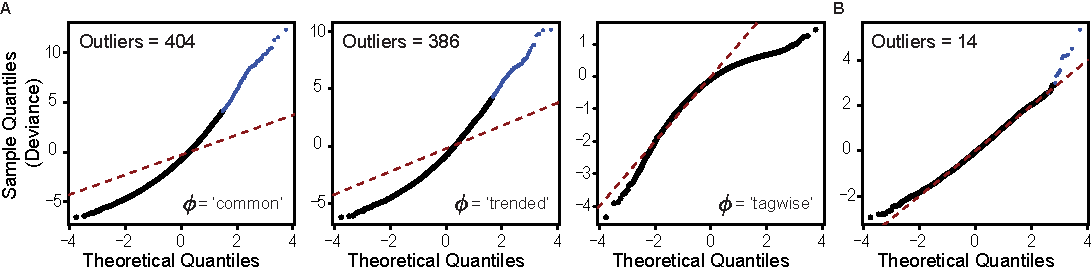
\includegraphics[width=0.9\paperwidth,keepaspectratio]{gof}
		\caption{\textbf{Goodness-of-fit of \texttt{edgeR} (A), and 
		\texttt{MSstatsTMT} (B) statistical approaches.} The overall
		adequacy of the linear models fit to the data were assessed 
		by plotting the residual deviance for all proteins as a 
		quantile-quantile plot (McCarthy \textit{et al.}, (2012)). 
		\textbf{(A)} For analysis with \texttt{edgeR}, The normalized
		protein data from \texttt{MSstatsTMT} were fit with a negative
		binomal generalized linear model (NBGLM) of the form: 
		\texttt{Abundance} $\sim$ \texttt{Mixture + Condition}.
		Where \texttt{Mixure} is an additive blocking factor that 
		accounts for variablity between experiments. 
		The NB framework used by edgeR utilizes a dispersion parameter 
		to account for mean-variance relationships in the data.
		The dispersion parameter can take several forms. 
                \texttt{edgeR} supports three dispersion models: 'common',
		'trended', and 'tagwise'. However, when using \texttt{edgeR's}
		robust quasi-likelihood test methods, only global (i.e. 'common'
		or 'trended') dispersion metrics are appropriate 
		(see \texttt{edgeR::glmQLFit's} documentation). 
		We plot the protein-wise deviance from the data fit withe ach of
		the disperions parameters. Protein-wise deviance
		statistics were transformed to normality and plotted against
		theoretical normal quantiles using the \texttt{edgeR::gof}
		function. \textbf{(B)} For analysis with \texttt{MSstatsTMT},
		the normalized protein data were fit with a linear mixed-effects 
		model (LMM) of the form: 
		\texttt{Abundance} $\sim$ \texttt{0 + Condition + (1|Mixture)}. 
		Where \texttt{Mixture} represents the random effect
		of \texttt{Mixture}. The residual deviance and degrees of 
		freedom were extracted from the fitted models, z-score
		normalized, and plotted as in (A). Proteins with a significantly 
		poor fit are indicated as outliers in blue 
		(Holm-adjusted P-value $<$ 0.05).}
		\label{fig:gof}
	\end{center}
	\end{fullwidth}
\end{figure}

%% MSstatsTMT
Of note, most tools for analysis of protein mass spectromety data are derived
from tools originally developed for analysis of genomics and transcriptomics
data. An exception to this norm is \texttt{MSstatsTMT}, an extension of 
\texttt{MSstats} for analysis of TMT proteomics experiments. \\

\texttt{MSstatsTMT} utilizes a linear mixed-model framework. The strength of 
linear mixed models (LMMs) is in their ability to account for complex sources of 
variation in an experimental design. \textbf{Figure \ref{fig:variance}} shows
the proportion of variance attributable to major covariates for each protein. \\

Linear mixed models are an extension of linear models which include both
fixed and random effects. 
The response (protein abundance) is a function of both fixed and mixed effects.
In a mixed model, one or more of the covariates are a categorical variable 
representing experimental or observational "units" in the data set. 

Thus random effects in mixed models often reflect heirarchically organized data 
such as repeated measurments of individual subjects. 
In mixed models we account for the variation occurring among all of the 
lower level units of a particular upper level unit.

The distinction between fixed and mixed effects is often subtle. By definition
if the set of possible levels of the covariate is fixed and reproducible then
the factor is modeled as a fixed-effect parameter. In contrast, if the levels of
an observation reflect a random sampling of the set of all pssible levels then
the covariate is modeled as a random effect. 

Huang et al., describe a general linear mixed model framework for mass 
spectrometry experiments. A TMT proteomics experiment consists of the analysis of 
\texttt{m =1} ... \texttt{M} concatensions of isobarically labeled samples 
or \texttt{Mixtures}. Within a mixture, each TMT channel is dedicated to the 
analysis of \texttt{c = 1} ... \texttt{C} individual biological or treatment 
\texttt{Conditions} prepared from \texttt{b = 1} ... \texttt{B} biological 
replicates or \texttt{Subjects}. A single mixture may be profiled in 
\texttt{t = 1} ... \texttt{T} technical replicate mass spectrometry runs.  \\

The following mixed-effects model describes the response, the abundance of 
protein $Y_{mcbt}$, in an experiment composed of \texttt{M} mixtures, \texttt{T} 
technical replicates of mixture, \texttt{C} conditions, and \texttt{B} biological subjects. 

%% Full model
\begin{equation} \label{eq1}
	Y_{mcbt} = \mu + Mixture_m + TechRep(Mixture)_{m(t)} + Subject_b + 
	Condition_c + \epsilon_{mcbt}
\end{equation}

The model's constraints distinguish fixed and random components of 
variation in the response. \texttt{Mixture} is a mixed effect and 
represents the variation between TMT mixtures which is assumed to be random 
and normally distributed. \texttt{TechRep(Mixture)} represents random variation 
between replicate mass spectrometry runs of a same mixture. 
The term \texttt{Subject} cooresponds to each biological replicate of a 
condition and represents biological variation among the levels of each 
\texttt{Condition}. \\

The term $\epsilon_mtcb$,
is a random effect representing both biological and technical variation, 
quantifying any remaining error ($\sigma^2$), and is assumed to be independent 
and non-systematic (no mean variance). \\

If a component of the model is not estimable, it is removed. Thus, if there is
no technical replication of Mixture, the model is reduced to: \\

%% Reduced model - no technical replication of mixture
\begin{equation} \label{eq2}
	Y_{mcbt} = \mu + Mixture_m + Condition_c + \epsilon_{mc}
\end{equation}

In the reduced model, biological variation among individual subjects is 
captured by the term \texttt{Condition} and is thus ommited.

We prepared 7 \texttt{BioFractions} from 'Control' and 
SWIP\textsuperscript{P1019R} 'Mutant' mice. Thus, in our experiment, 
the fixed effect term condition represents interaction of \texttt{Genotype} and 
\texttt{BioFraction} and represents the 14 unique combinations 
of 7 subcellular \texttt{BioFractions} prepared from 'Control' and 'Mutant' mice. 

In our experimental design, we made seven repeated measurments 
from each biological Subject. Thus, the term Subject represents the random error
within a subject. However, in our design \texttt{Mixture} is confounded with the
term \texttt{Subject} -- in each mixture we analyzed all \texttt{BioFractions} 
from a single Control and Mutant mouse. Thus we can choose to account for the 
effect of \texttt{Mixture} or \texttt{Subject}, but not both. 
Assuming Mixture contributes greater to the variance, we drop the term Subject,
and the reduced model is equivalent  to \ref{eq2}. Our experimental design is 
summarized in \textbf{Figure \ref{fig:design}}.

\begin{figure}[h]
  \begin{fullwidth}
  \begin{center}
	  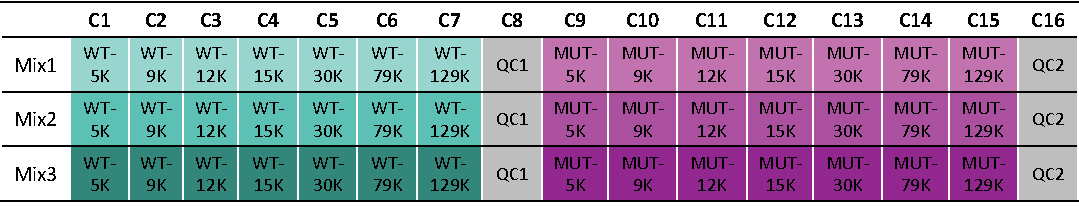
\includegraphics[width=0.9\paperwidth,keepaspectratio]{design}
	  \caption{\textbf{Experimental Design.} We performed three 16-plex TMT
	  experiments. Each TMT mixture is a concatenation of 16 labeled
	  samples. In each experiment we analyzed 7 subcellular
	  \texttt{BioFractions} prepared from the brain of a 'Control' or
	  'Mutant' mouse. In all we analyzed 3 \texttt{Subjects} from each 
	  {Condition}. Each \texttt{Mixture} includes two \texttt{Channels}
	  dedicated to the analysis of a common quality control sample.}
	  \label{fig:design}
  \end{center}
  \end{fullwidth}
\end{figure}

Model based testing of differential abundance between pairs of conditions
is assessed through contrast of conditioned means estimated by fitting the
parameters of the model by REML to obtain $\hat{\beta}$, $\sigma^2$ and
$\hat{V}$. A contrast or comparison between coefficients in the model is
specified by a vector of sum 1 which indicates the positive and negative
coefficients of the comparison \textbf{Figure \ref{fig:contrasts}}.

\begin{figure}[h]
  \begin{fullwidth}
  \begin{center}
	  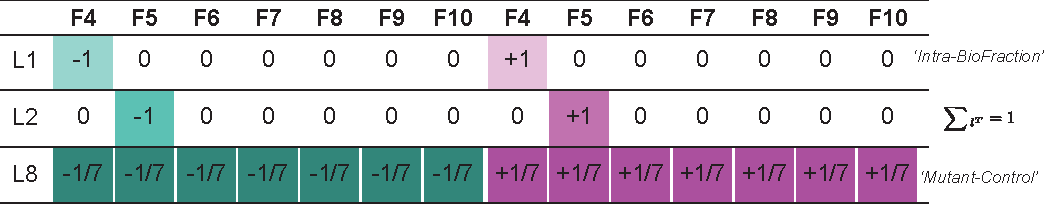
\includegraphics[width=0.9\paperwidth,keepaspectratio]{contrasts}
	  \caption{\textbf{Statistical Comparisons.} We assessed two types of
	  contrasts. Each row of the matrix specifies a contrast between
	  positive and negative coefficients in the mixed effects model fit to
	  each protein. Contrasts1-7 are 'intra-BioFraction' contrasts that
	  specify the pairwise comparisons of Control and Mutant groups for a
	  single fraction. In Contrast 8 we compare 'Mutant-Control' and asses
	  the overall difference of 'Control' and 'Mutant' conditions.  Each
	  contrast is a vector of sum 1.}
	  \label{fig:contrasts}
  \end{center}
  \end{fullwidth}
\end{figure}


The degrees of freedom are determined by the Satterthwaite approximation
and the T-statistic for the contrast is taken to be (lmerTest ref): \\

%% T-statistic Equation
\begin{equation}
	t = \frac{l^T * \hat{\beta}}{sqrt(l * \sigma^2 * \hat{V} * l^T)}
\end{equation}

Where $\sigma^2$ is the error from \textbf{Equation} \ref{eq1}.
$l^T$ is a vector specifying a contrast between positive and 
negative coefficients in the model.

Together, the denominator $\sqrt(l * \sigma^2 * \hat{V} * l^T)$ is the 
standard error of the contrast.

%%

We reanalyzed the data with \texttt{MSstatsTMT} starting with PSM-level data 
exported from ProteomeDiscoverer. The intial dataset was composed of 8,590 
unique proteins. The PSM level data are converted to MSstatsTMT's format 
and protein summarization and normalization is performed using the QC samples. 

Reprodcible quantification of these samples is essential. Thus we examined PSM features for potential outliers, accounting for the mean-variance relationship in 
PSM quantification using the method described by Plubell et al. (REF).

We removed PSM with incomplete observations from each experiment 
(n=186, 132, and 174 respectively from each of the three mixtures).

A small number of QC outliers were identified and removed (M1=259; M2=169;
M3=159). \\

We performed protein-level normalization and sumamrization using
\texttt{MSstatsTMT}. This step is computationally expensive as each protein is
fit with a linear model. We increased the efficiency of this computation by
employing 23 parallel processors, in all taking approximately 11.094 minutes.

MSstatsTMT takes care to impute missing values within each Run. But missing
values still exist at the protein level. In order to avoid discarding a large
number or proteins we impute these missing values using the KNN algorithm for
MNAR data. This does not affect the statistical testing, but helps retain
proteins used to build the covariation network.
Porieins with more than 50\% missingness cannot be reliably imputed and are
removed (66 rows). In all we retained 6,910 of the inital 8,590 proteins in the 
final normalized dataset.  \\

We assess protein-level comparisons at two different levels using MSStatsTMT.
We asses 'intra-BioFraction' comparisions and moderated these test statistics 
for small sample size (n=3 for each condition).
This step is computationally expensive as a linear-mixed model is fit to each
protein in the data. The time to perform intra-Biofraction comparisons for all 
proteins was approximately 17.834 minutes. \\

We assed overall differnces between 'Mutant' and 'Control' conditions using
MSstatsTMT (Moderated=FALSE). \\

There were 163 instances of signficant differential abundance for 
'intra-BioFraction' comparisons (FDR < 0.05). The following table summarizes 
the number of significantly differential abundant
proteins for each of the seven intra-BioFraction comparisons. \\

%```
%| F4| F5| F6| F7| F8| F9| F10|
%|--:|--:|--:|--:|--:|--:|---:|
%| 17| 22| 20| 27| 28| 27|  22|
%```

There were 785 proteins with an overall significant change for the
'Mutant-Control' comparison.

%% Network Construction

Prior to building the protein covariation network, we removed the effect of
Mixture using limma::RemoveBatchEffect. This is necessary as we wish to identify
modules that covary together across subcellular space (BioFraction) and not
batch or Mixture.  These adjusted data are used for network construction and
plotting but not statistical modeling. It is preferable to include these factors
in the statistical model.

The final, tidy normalized protein data is avaialbe as an R object, 
\texttt{msstats\_prot} in \texttt{SwipProteomics/data}.

We extracted MSstatsTMT's core model-fitting and statistical testing steps. It
is usefull to allow investiagors flexiblity and transparency. 

We evaluate the percent variance explained by each factor in the LMM using the
\texttt{variancePartition} package.


%% Assessing Goodness of fit.

We assessed the goodness-of-fit of each protein-wise LMM using Nagagawa's
coefficient of determination, as implemented by the 
\texttt{r.squaredGLMM.merMod} function forked from the \texttt{MuMin} package.

Prior to network construction, we removed models with poor fit. We removed
proteins whose model explained less than 0.7 of the variation for that protein. 

%| r2_threshold| out| percent| total| final|
%|------------:|---:|-------:|-----:|-----:|
%|          0.7| 791|   0.114|  6910|  6119|

Number of proteins with poor fit: 791

Removing this small number of proteins facilitates clustering.

% WASHC* protein goodness-of-fit statistics:
%|Protein |Symbol | Entrez|   Mixture|  Genotype| BioFraction| Residuals|  R2.fixef|  R2.total|
%|:-------|:------|------:|---------:|---------:|-----------:|---------:|---------:|---------:|
%|Q8C2E7  |Washc5 | 223593| 0.0004987| 0.9130491|   0.0442397| 0.0422125| 0.9744804| 0.9762336|
%|Q8VDD8  |Washc1 |  68767| 0.0070136| 0.8808449|   0.0436028| 0.0685388| 0.9232585| 0.9298346|
%|Q3UMB9  |Washc4 | 319277| 0.0133109| 0.8722170|   0.0489876| 0.0654845| 0.9353344| 0.9494330|
%|Q6PGL7  |Washc2 |  28006| 0.0000000| 0.7646015|   0.1685491| 0.0668494| 0.9409087| 0.9409087|
%|Q9CR27  |Washc3 |  67282| 0.0205066| 0.6701031|   0.0640885| 0.2453017| 0.7341464| 0.7521275|

Removing 791 proteins with poor fit before building network. 
The final network was constructed using both 'Control' and 'Mutant' samples. The
data adjsuted for batch (Mixture). It contained 42 samples and 6,119 proteins.
We found that the pearson correlatioin statistic outperformed the bicor
statistic we previously used. \\

%
%| samples| proteins|
%|-------:|--------:|
%|      42|     6119|

%% Generating protein co-variation network.

We performed network enhancement to remove biological noise from the datset.
This step is essential for module detection. Our approach borrows many of the
conceptual ideas utilized in the WGCNA or WPCNA analysis workflows. Network
enhancement is analogous to the weighting step performed by WGCNA and analogous
emthods in which the network correlation network is transformed by a power in
order to re-weight the network. Network enhancment has the effect of making the
network sparse and facilitates the identification of network structure.

We constructed a protein-protein interaction graph which was not used to guide
clukstering, but as an additional layer of information in the final network
graphs. The PPI graph for all proteins contained 93,573 edges.

%% Quality Metric

We sought to identify groups, aka clusters or modules, of proteins that strongly
covary together across subcellular space. Intuitively, we wish to identify a
partition of the graph which maximizes intra-module connectivity and minimizes 
inter-module connectivity. Numerous quality statistics descriving the overall
quality of a network partition exist, and numerous heuristical algorithms.

Identification of communities in a graph by optimization of a quality function
is NP-hard5, and consequentially many heuristic algorithms exist.
One of the most well known algorithms, is the Louvain algorithm
(Traag2010ref10).  \\

We utilized a recent improvement of the Louvain algorith, the 
Leiden algorithm to identify optimal partitions of the graph. 
The Leiden algorithm is implemented in Python and supports several quality
statistics, including Modularity, CPM, Surprise, RBER, and RBConfiguration.

We aim to cluster the protein-covariation network in order to identify modules
which cohesive protein abundance profiles.

For each model fit the module-level data, we asses the proprotion of variance
explained by BioFraction, Genotype, Mixture, and Protein using the
\texttt{VariancePartition} R package. We also compute Nagakawa's coefficient of
determination for mixed models, as implemented by the R \texttt{MuMin} package. 
Inspection of these variance explained by the components of our model we 
realize a natural description of a modules quality. 

R2(fixef) aka R2c (conditional) -- interpretation: the total variance explained
by fixed effects (Genotype:BioFraction). We wish to maximize this quantity.

PVE(protein) -- the percent of the modules variation explained by protein
variability. An ideal module is a perfect summary of its constituent proteins
and this quantity is 0. We aim to minimize the PVE(protein).

An ideal module is a perfect summary of its constituent proteins. Thus, we seek
to minimize the variation arising from Protein within a module. While minimizing
this quantity, we aim to retain clusters whose variation attributed to fixed
effects of BioFraction and Genotype is maximized. Thus, a simple quality metric
for a module may be the ratio of variance attributable to fixed effects and the
random effect of protein:

%q_k = PVE(fixef) / PVE(protein)
%This is equivalent to:
%q_k = var(fixef) / var(protein)

The overall quality of a partition is the average all module quality.

All things being equal, an increase in the number of clusters results in a
decrease in overall quality. (Imagine splitting a perfect module,into two; for
each the variance attributed to Protein is 0, but when this module is split the
variance attributable to each modules fixed effects is halved).

Performing Leidenalg clustering utilizing the 
SurpriseVertexPartition method to find optimal partition(s).

Recursively splitting modules larger than 100 nodes with 'Surprise'.
We find that recursive splitting of large modules is necessary to resolve 
significant heterogenity which exists in large modules and this also improves 
recovery of biological signal.

We split modules with more than 100 nodes. While this threshold is arbitrary, we
found that recursively spliting large modules resulted in higher quality
modules. and facilitates biological indference.

Final partition:  Clustering with 6119 elements and 502 clusters
We removed small mdoules of less than 5 nodes.

Module statistic(s) used to evaluate module  preservation:
avg.weight, avg.cor, avg.contrib.
Criterion for module preservation: strong.

We enforced module quality by module preservation using a permutation appraoch.
Modules with random toplogy we discarded. 


Evaluating  preservation of Swip modules in the Swip network...
... 296 of 329 Swip modules are preserved in the Swip network.

In all there were 296 modules.

%|nProts |kModules |pClustered |medSize |
%|:------|:--------|:----------|:-------|
%|6,119  |296      |0.908      |13      |


%|Term                   | Estimate|    SE|    DF| Tvalue|Pvalue    |
%|:----------------------|--------:|-----:|-----:|------:|:---------|
%|Control:BioFractionF4  |    6.883| 0.151| 6.891| 45.636|2.91e-09  |
%|Control:BioFractionF5  |    7.167| 0.151| 6.891| 47.520|8.249e-10 |
%|Control:BioFractionF6  |    7.465| 0.151| 6.891| 49.494|2.289e-09 |
%|Control:BioFractionF7  |    7.495| 0.151| 6.891| 49.692|6.248e-10 |
%|Control:BioFractionF8  |    7.327| 0.151| 6.891| 48.580|2.017e-09 |
%|Control:BioFractionF9  |    7.138| 0.151| 6.891| 47.328|4.722e-10 |
%|Control:BioFractionF10 |    7.756| 0.151| 6.891| 51.424|1.931e-09 |
%|Mutant:BioFractionF4   |    5.729| 0.151| 6.891| 37.983|4.595e-10 |
%|Mutant:BioFractionF5   |    5.933| 0.151| 6.891| 39.334|2.303e-09 |
%|Mutant:BioFractionF6   |    6.043| 0.151| 6.891| 40.065|5.369e-10 |
%|Mutant:BioFractionF7   |    6.082| 0.151| 6.891| 40.322|2.384e-09 |
%|Mutant:BioFractionF8   |    5.927| 0.151| 6.891| 39.299|6.424e-10 |
%|Mutant:BioFractionF9   |    5.897| 0.151| 6.891| 39.101|1.991e-09 |
%|Mutant:BioFractionF10  |    6.054| 0.151| 6.891| 40.142|3.631e-10 |


Nakagawa coefficient of determination
R2m: Marginal; variation explained by fixed effects.
R2c: Conditional; total variation explained by the model.


%|       R2m|       R2c|
%|---------:|---------:|
%| 0.7620866| 0.8928053|


%|Contrast       |    log2FC| percentControl| Pvalue| Tstatistic|        SE|  DF| nProteins|
%|:--------------|---------:|--------------:|------:|----------:|---------:|---:|---------:|
%|Mutant-Control | -1.366663|      0.3877871|      0|  -36.94728| 0.0369896| 190|         5|

Assessing module-level contrasts with lmerTest.

Time to analyze 296 modules:
Time difference of 5.151603 secs

Final number of modules : 296

Final percent clustered : 0.908

Final Median module size: 13

Washc4 assigned to module: M17

All significant (Padjust < 0.05) modules:

Number of significant modules (Bonferroni<0.05): 61

Evaluating goodness-of-fit of modules.
There were problems fitting 0 models.

Partition Quality: 2.14995 (mean module quality).

%% Module goodness-of-fit statistics.
The Columns BioFraction Genotype, Mixture, Protein, and Residuals describe the
percent variance attributable to that term for the mixed-effect model fit to
each module. R2.fixef is the overall variance explained by fixed effects.
R2.total is the overall variance explained by the model.
An intuitive measure of module quality is the ratio of variance explained by
fixed effects and Protein. We wish to maximize the variance explained by fixed
effects and minimize the random effect of Protein. An ideal module is a perfect
summary of its protein constituents and thus PVE(Protein) = 0. 


Number of modules with something interesting going on: 116

Significant Modules with significant gse:
(23 of 61 significant modules.)

%## Modules with significant LopitDC gse:
%Top module for each LopitDC category

%|Pathway                    |TopModule |        FE|   Padjust|
%|:--------------------------|:---------|---------:|---------:|
%|LopitDC: CYTOSOL           |M52       |  8.992783| 0.0000000|
%|LopitDC: ER                |M72       | 11.314516| 0.0000000|
%|LopitDC: GA                |M285      | 54.540444| 0.0000000|
%|LopitDC: LYSOSOME          |M3        | 17.729026| 0.0000000|
%|LopitDC: MITOCHONDRION     |M32       |  9.618624| 0.0000000|
%|LopitDC: NUCLEUS/CHROMATIN |M97       |  4.368595| 0.0000000|
%|LopitDC: PEROXISOME        |M239      | 74.895623| 0.0000000|
%|LopitDC: PM                |M199      | 10.921082| 0.0002154|
%|LopitDC: PROTEASOME        |M83       | 62.153846| 0.0000000|
%|LopitDC: RIBOSOME          |M119      | 29.597031| 0.0000000|

\end{document}
